\documentclass{article}

\usepackage[a4paper,margin=1in]{geometry}

\usepackage{hyperref}
\usepackage[utf8]{inputenc}
\usepackage[english]{babel}
\usepackage{textpos}
\usepackage{textcomp}
\usepackage{amsmath}
\usepackage{amssymb}
\usepackage{amsfonts}
\usepackage{graphicx}
\usepackage{epstopdf}
\usepackage{algorithmic}
\usepackage{verbatim}
\usepackage{textcomp}
\usepackage{varwidth}
\usepackage[linesnumbered,ruled]{algorithm2e}
\usepackage{multicol}
\usepackage{palatino}

% For displaying code
\usepackage{listings}

\usepackage{enumitem}
% Change format of top-level list items
%\setlist[enumerate,1]{label*=\arabic*,font=\bfseries,before=\bfseries}
% Reset formatting for subsequent levels; label type makes 1.1, legal-style labels
%\setlist[enumerate,2]{label*=.\arabic*,font=\normalfont,before=\normalfont}

% Theorem
\newtheorem{theorem}{Theorem}

% lists
\usepackage{outlines}
\usepackage{enumitem}
\newenvironment{tight_enum}{
\begin{enumerate}[label=\alph*.]
\setlength{\itemsep}{0pt}
\setlength{\parskip}{0pt}
}{\end{enumerate}}

% \subsubsubsection{}
\setcounter{secnumdepth}{5}
\setcounter{tocdepth}{5}
\newcommand\simpleparagraph[1]{%
  \stepcounter{paragraph}\paragraph*{\theparagraph\quad{}#1}}

\usepackage{color}
\usepackage{xcolor}
\usepackage{mdframed}

\definecolor{dkgreen}{rgb}{0,0.6,0}
\definecolor{gray}{rgb}{0.5,0.5,0.5}
\definecolor{mauve}{rgb}{0.58,0,0.82}

% \usepackage{courier}
\lstset{%frame=tb,
language=C++,
aboveskip=3mm,
belowskip=3mm,
showstringspaces=false,
columns=flexible,
basicstyle={\small\ttfamily},
numbers=none,
numberstyle=\tiny\color{gray},
keywordstyle=\color{blue},
commentstyle=\color{dkgreen},
stringstyle=\color{mauve},
breaklines=true,
breakatwhitespace=true,
tabsize=3
}

\newtheorem{definition}{Definition}



%%%%%%%%% BEGIN DOCUMENT %%%%%%%%%
%%%%%%%%% BEGIN DOCUMENT %%%%%%%%%
%%%%%%%%% BEGIN DOCUMENT %%%%%%%%%

%% Used tt when referring to function

\begin{document}

\title{Engineerging Programming II: \\ Random Number Generation}
\author{Graham West}
\date{}

\maketitle

\large

\tableofcontents

\begin{comment}

\begin{algorithm}[h!]
	\begin{algorithmic}[1]
		\FOR{ $n = 1$ \TO $N_{gen}$}
			$(x_i,y_i)$ where
		\ENDFOR
	\end{algorithmic}
	\caption{test}
\end{algorithm}

\end{comment}


%%%%%%%%%%%%%
%%% NEW SECTION %%%
%%%%%%%%%%%%%
\section{Random variables}

Let us start with the definition of a random variable. A \textbf{random variable} $X$ is a quantity that can ``randomly'' take on any of a number of different values. The set of possible values it can assume (i.e., the set of possible \textbf{outcomes}) is called the \textbf{sample space}, often denoted $S$. Consider the simple example of flipping a coin. In this case, $S=\{$heads, tails$\}$, so a random variable drawn from this sample space could assume outcomes of either \emph{heads} or \emph{tails}. Now, we must also define a \textbf{probability distribution} $P$ over this sample space so that we can determine the likelihoods of the outcomes \footnote{Technically, $P$ is a \textbf{measure} on $S$, meaning it is defined on \emph{subsets} of $S$, not elements ot it. However, it is common to abuse notation and talk about $P(X)$ as opposed to $P(\{X\})$.}. 




%%%%%%%%%%%%%
%%% NEW SECTION %%%
%%%%%%%%%%%%%
\section{Drawing from distributions in Python}

\begin{enumerate}
	\item Random integer
	\item Choice
	\item Uniform
	\item Normal
	\item Multivariate normal
\end{enumerate}



%%%%%%%%%%%%%
%%% NEW SECTION %%%
%%%%%%%%%%%%%
\section{Uniform distributions over specific domains}

\subsection{Rectangle}

It is very easy to create a uniform distribution over a rectangle (or high-dimensional analogue). For example, if we wanted to sample a uniform distribution over the rectangle $[0,2]\times[0,1]$, we can construct points $(x_i,y_i)$ where $x_i \sim U(0,2)$ and $y_i \sim U(0,1)$ for all $i$. See Figure \ref{UniRect} for an illustration of this.
\begin{figure}[h]
	\centering
	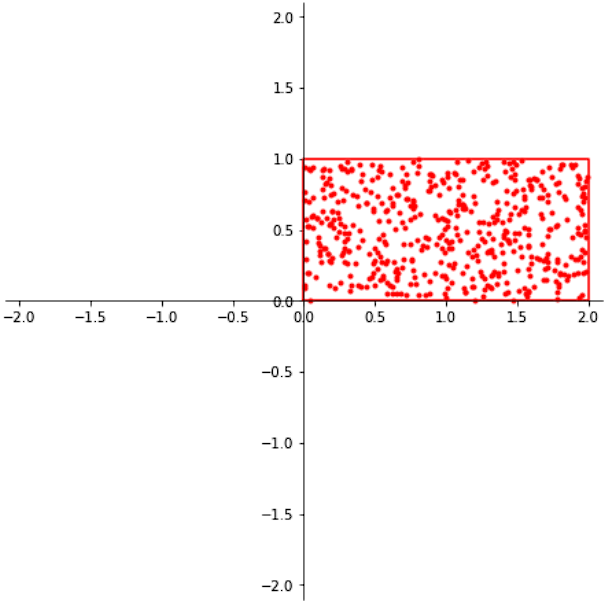
\includegraphics[width=0.5\linewidth]{UniformRectangle}
	\caption{Uniformly sampled points from $[0,2]\times[0,1]$.}
	\label{UniRect}
\end{figure}

\subsection{Circle}

However, generating uniformly sampled points from, say, a circle is slightly more involved. We cannot simply define the bounds on four edges. We must be more clever. The problem can be solved by using \emph{polar coordinates}, i.e., we generate angles $\theta$ and radii $r$ for the points. Let us try to uniformly sample points from a circle of radius 1 centered on the origin.

\begin{mdframed}[backgroundcolor=red!20]
\textbf{THE WRONG WAY}

\vspace{10pt}

It should be immediately noted that there is a mistake that is all too easy to make. At first glance, one might think that we can simply draw $\theta_i \sim [0,2\pi)$ and $r_i \sim [0,1]$. Doing this causes the distribution to be more dense in the center since it ignores the fact that the ``ring's'' of constant $r$ around the circle get longer in circumference as they get further from the center. Thus, a ring of constant $r$ close to the center will have just as many points as a ring far from the center despite the fact that it is shorter. See the left graph in Figure \ref{UniCirc} for an illustration.
\end{mdframed}

\begin{mdframed}[backgroundcolor=green!20]
\textbf{THE RIGHT WAY}

\vspace{10pt}

To fix this we simply draw $\theta_i \sim [0,2\pi)$ and $r_i^2 \sim [0,1]$ (or, $r_i = \sqrt{\hat r_i}$ where $\hat r_i \sim [0,1]$). In other words, we take the square root of the random number we draw. Doing this accounts for the increasing circumference of the rings of constant $r$. See the right graph in Figure \ref{UniCirc} for an illustration.
\end{mdframed}

\begin{figure}[h]
	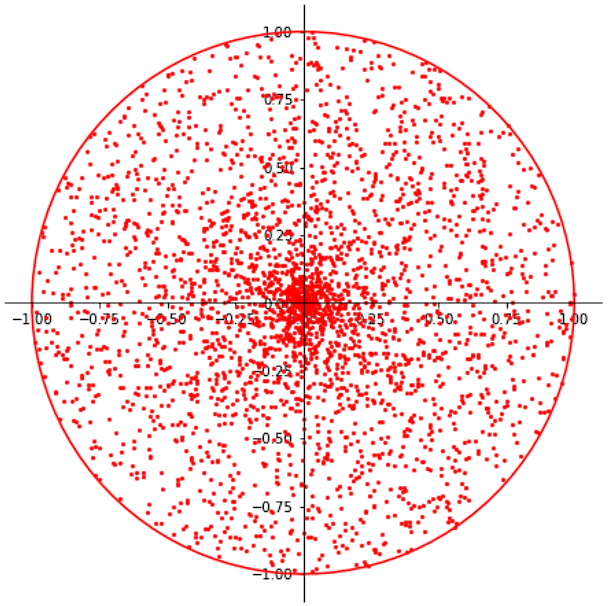
\includegraphics[width=0.5\linewidth]{UniformCircle_Wrong}
	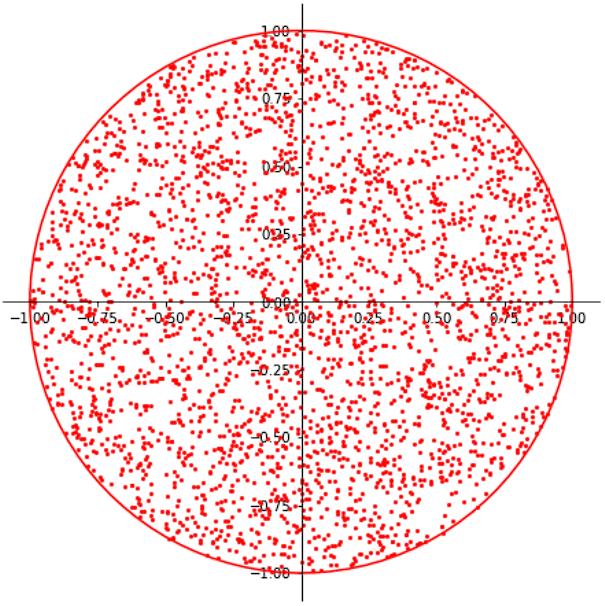
\includegraphics[width=0.5\linewidth]{UniformCircle_Right}
	\caption{Left: failing to uniformly sample the circle. Right: correctly uniformly sampling the circle.}
	\label{UniCirc}
\end{figure}





%%%%%%%%%%%%%
%%% NEW SECTION %%%
%%%%%%%%%%%%%
\section{Homework}

\subsection{Random walk on plane}

\subsection{Uniform distribution on a cylinder}

\subsection{Uniform distribution on a sphere}

scale by cos

\subsection{Random walk on sphere}




\end{document}
